\section{Shared caching layer between micro-frontends}\label{section:applied-methods:shared-caching-layer}

\noindent With the help of the learnings from the previous Section \ref{section:applied-methods:communication-shell-remote} on how to communicate between micro-frontends, a shared caching layer should be implemented. This section describes how the shared caching layer was developed and how it can be used inside the application. The structure of the shared caching layer should look like in the Figure \ref{fig:applied-methods:structure-shared-caching-layer}. The micro-frontends have a separate instance of the Apollo Client, but they should all use the same instance of the in-memory cache. Therefore, each application can provide configuration for the Apollo Client, but they all use the same instance of the cache. The in-memory cache stores the results of the GraphQL queries. If the micro-frontends need to fetch the same query with the same data, they can use the data already stored in the cache instead of fetching it from the server again. The approach reduces the number of network requests and, therefore, the amount of data that has to be transferred over the network. 

\ifshowImages
  \begin{figure}[H]
  \centering
  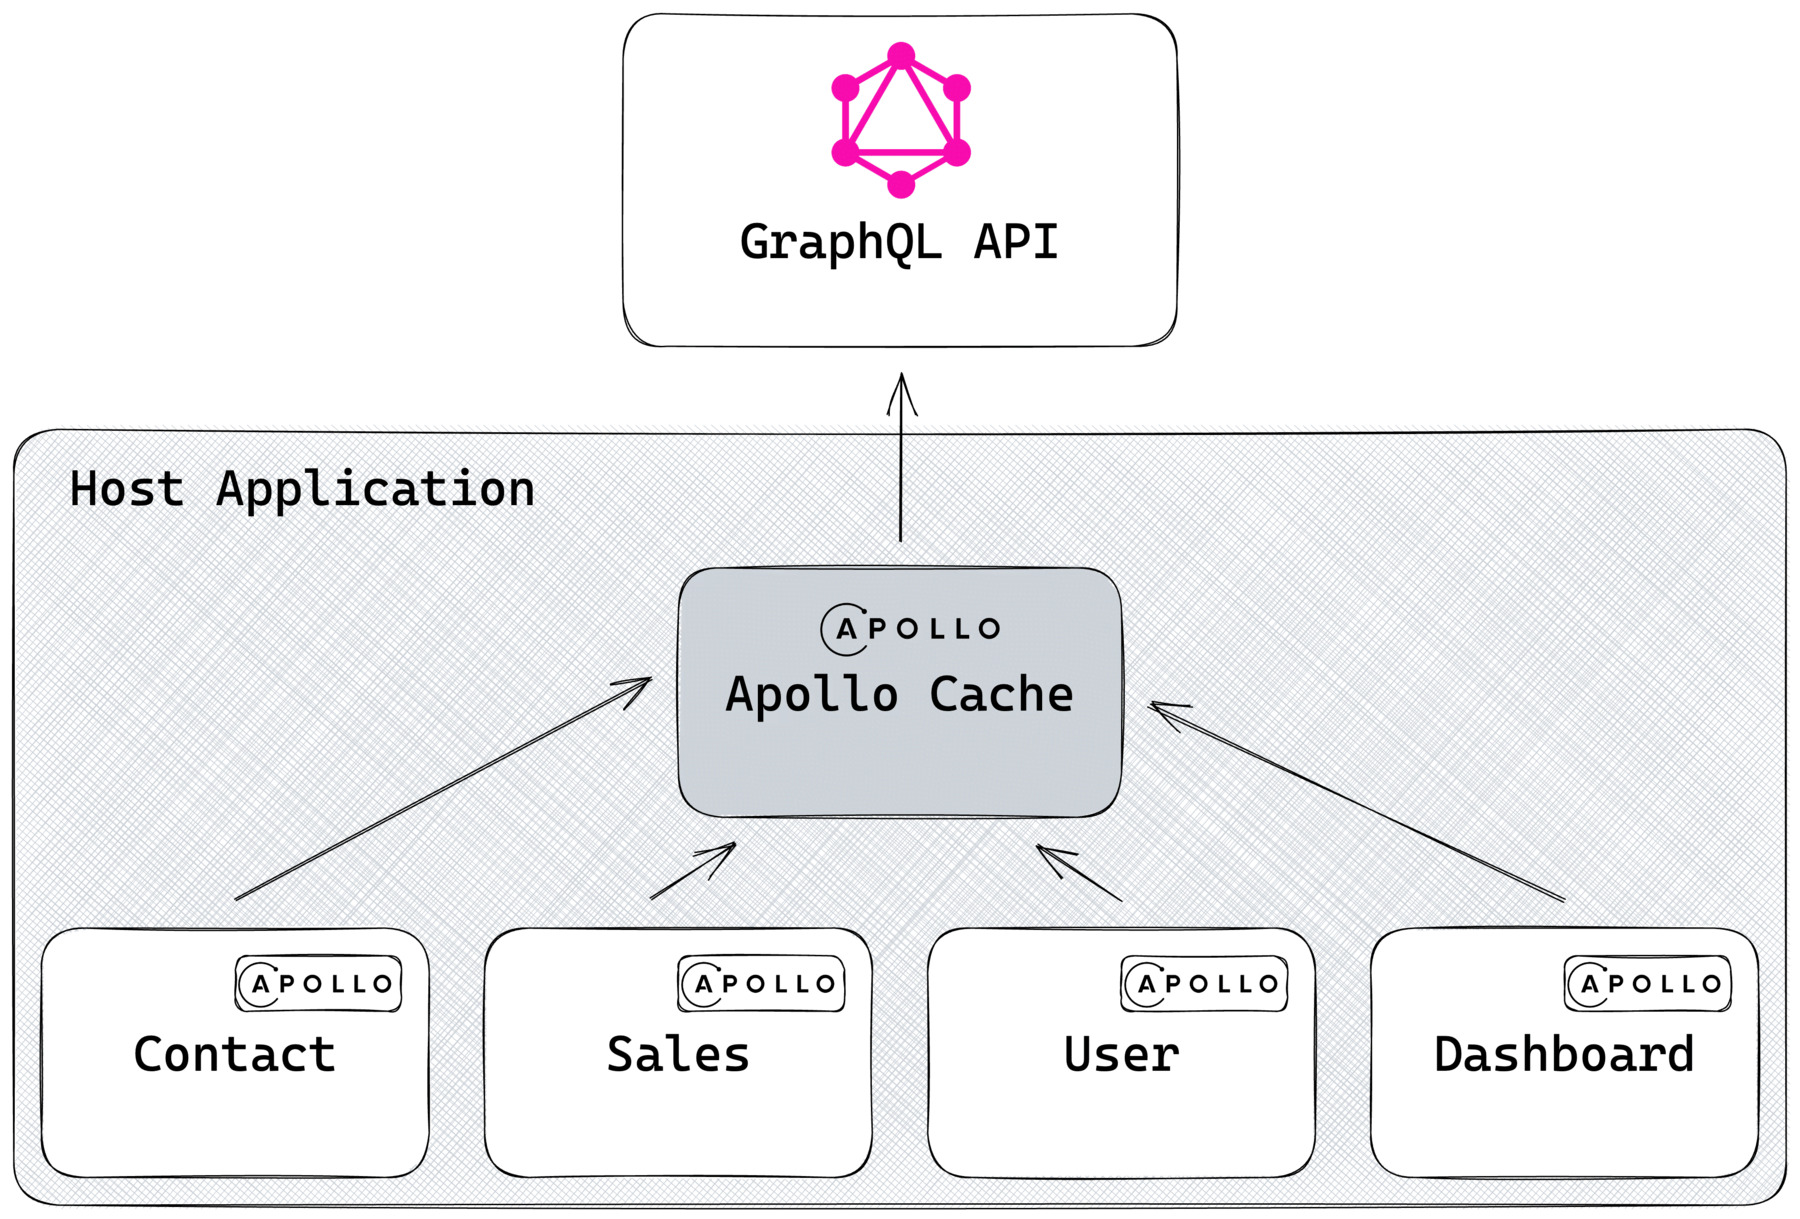
\includegraphics[width=0.8\linewidth]{images/applied-methods/shared-caching-layer/shared-caching-layer.jpg}
  \caption{The structure of the shared caching layer.}\label{fig:applied-methods:structure-shared-caching-layer}
  \end{figure}
\fi

\noindent The application shell should provide the instance of the GraphQL \texttt{InMemoryCache}. The Listing \ref{code:applied-methods:creating-the-apollo-client} shows how the Apollo Client is created in Angular for an application with default settings. The \texttt{cache} property is important, as it needs an instance of Apollo's \texttt{InMemoryCache}. This allows for the architecture to create a cache instance elsewhere and pass it to the Apollo Client. 

\ifshowListings
\begin{listing}[H]
\begin{minted}{typescript}
@NgModule({
  imports: [ApolloModule],
  providers: [{
    provide: APOLLO_OPTIONS,
    useFactory: (httpLink: HttpLink) => ({
      cache: new InMemoryCache(),
      link: httpLink.create({ uri: 'http://localhost:3000' }),
    }),
    deps: [HttpLink],
  }]
})
class AppModule {}
\end{minted}
\caption{Create a new instance of the Apollo Client.}\label{code:applied-methods:creating-the-apollo-client}
\end{listing}
\fi

\noindent The idea is to instantiate the cache instance inside the application shell and provide it to the remote applications. The instance of the in-memory cache should be provided through an injection token, just like the injection token from the communication Section \ref{section:applied-methods:communication-shell-remote}, that specifies whether the application is consumed by the application shell or the application runs in standalone mode. The injection token can be provided by the application shell and injected by the remote modules of the micro-frontends. Moreover, the application itself can provide the token when it runs in standalone mode. The \texttt{InMemoryCache} provider can be implemented by providing the instance of the cache through an injection token called \texttt{GRAPHQL\_CLIENT\_CACHE}, as shown in the Listing \ref{code:applied-methods:graphql-client-cache-provider}.

\ifshowListings
\begin{listing}[H]
\begin{minted}{typescript}
@NgModule({
  providers: [
    { provide: GRAPHQL_CLIENT_CACHE, useValue: new InMemoryCache() }
  ]
})
class HostCoreModule {}
\end{minted}
\caption{Provide the instance of the \texttt{InMemoryCache} to \ac{DI}.}\label{code:applied-methods:graphql-client-cache-provider}
\end{listing}
\fi

\subsection{GraphQL Client creation}

\noindent The prototypical micro-frontend architecture implements abstractions to create the necessary configuration for the Apollo Client more easily and identically for all micro-frontends. Listing \ref{code:applied-methods:graphql-client-creation} shows the abstraction to create a GraphQL client for a micro-frontend. The function provides the module, which imports the \texttt{GraphQLClientOptionsModule}, with an instance of the Apollo Client. The function takes one required parameter that specifies a unique name for the GraphQL client. The client's name is used to identify active Apollo Clients inside the architecture. The \texttt{GraphQLClientOptionsModule} encapsulates the steps to create an Apollo Client, as shown in the Listing \ref{code:applied-methods:creating-the-apollo-client-with-a-shared-cache}. The \texttt{GraphQLClientOptionsModule} should be used in every module that uses GraphQL and is exposed through Module Federation. If the remote module is then used inside the application shell, it has its separate Apollo Client. That makes the independent development of the micro-frontends easier because the Apollo Client's settings will be the same, regardless if it is running in standalone mode or is consumed by the application shell. For example, a problem would be if the application shell provides the Apollo Client and the contact micro-frontend injects that instance with \ac{DI}. The contact development team might configure the Apollo Client differently inside the contact application, and the functionality might not work as expected inside the application because the configuration may be different.

\ifshowListings
  \begin{listing}[H]
    \begin{minted}{typescript}
@NgModule({
  imports: [ GraphQLClientOptionsModule.withConfig('contact-remote') ]
})
class ContactRemoteCoreModule {}
  \end{minted}
  \caption{Create the Apollo Client instance for the micro-frontend.}\label{code:applied-methods:graphql-client-creation}
  \end{listing}
\fi

\ifshowListings
\begin{listing}[H]
\begin{minted}{typescript}
@NgModule({
  imports: [ApolloModule],
  providers: [{
    provide: APOLLO_OPTIONS,
    useFactory(httpLink: HttpLink, cache: InMemoryCache) {
      const link = httpLink.create({uri: 'http://localhost:3000'});
      return { cache, link };
    },
    deps: [HttpLink, GRAPHQL_CLIENT_CACHE],
  }]
})
class ContactRemoteModule {}
\end{minted}
\caption{Access the shared \texttt{InMemoryCache} instance from \ac{DI}.}\label{code:applied-methods:creating-the-apollo-client-with-a-shared-cache}
\end{listing}
\fi

\noindent The function creates a new Apollo Client instance with specified default settings. The \ac{URL} of the GraphQL \ac{API} is taken from the storage service. By default, it tries to inject the \texttt{GRAPHQL\_CLIENT\_CACHE}, to use a shared cache instance. If it cannot be injected, it creates a separate cache instance for the client. An injection token named \texttt{GRAPHQL\_CLIENT\_OPTIONS\_CONFIG} can be used to specify further options when creating an Apollo Client inside the micro-frontend architecture. The injection token's usage and default options are shown inside Listing \ref{code:applied-methods:graphql-client-extra-configuration-options}. The injection token must be specified inside the same module where the \texttt{GraphQLClientOptionsModule} was defined.

\ifshowListings
\begin{listing}[H]
\begin{minted}{typescript}
@NgModule({
  providers: [{
    provide: GRAPHQL_CLIENT_OPTIONS_CONFIG,
    useValue: {
      shareCache: true,
      persistCache: false,
      useTypePolicies: true,
      typePolicies: CONTACT_TYPE_POLICIES,
    },
  }]
})
class ContactRemoteCoreModule {}
\end{minted}
\caption{Provide additional options for creating the Apollo Client instance.}\label{code:applied-methods:graphql-client-extra-configuration-options}
\end{listing}
\fi

\noindent The options include \texttt{shareCache}, \texttt{persistCache}, \texttt{useTypePolicies} and \texttt{typePolicies}. \texttt{shareCache} is used to specify if the Apollo Client should use the in-memory cache instance provided by \texttt{GRAPHQL\_CLIENT\_CACHE} or if it should create a new instance, specifically for this remote module. The \texttt{persistCache} option is set to \texttt{false} by default. It stores the contents of the in-memory cache inside the \texttt{localStorage}. This feature provided by the Apollo Client allows faster initial page renders, because the data from the \texttt{localStorage} is transferred back to the cache when the application is loaded. The options \texttt{useTypePolicies} and \texttt{typePolicies} are used together and must be specified together. The property \texttt{useTypePolicies} specifies whether the type policies from the option \texttt{typePolicies} should be used or not. Type policies allow Apollo Client to customize the read and write operations for the cache. They are explained in more detail in Section \ref{subsubsection:background:graphql:apollo-server-client:type-policies}. As explained before every micro-frontend has a separate Apollo Client instance, with a shared cache instance, therefore, the type policies cannot be registered directly when creating the \texttt{InMemoryCache}. The option \texttt{typePolicies} is typed identical to the parameter \texttt{typePolicies} of the \texttt{InMemoryCache} constructor. Specifying the option when providing the \texttt{GRAPHQL\_CLIENT\_OPTIONS\_CONFIG} allows the micro-frontend to specify additional type policies for the cache. Part of the code of the abstraction to create the Apollo Client inside the \texttt{GraphQLClientOptionsModule} is shown in Listing \ref{code:applied-methods:adding-extra-type-policies}. First, the instance of the cache is injected. If the cache cannot be injected, it means that the Apollo Client should create and use a new instance of the cache. The \texttt{typePolicies} are added to the cache if the options \texttt{typePolicies} and \texttt{useTypePolicies} are both truthy values.

\ifshowListings
\begin{listing}[H]
\begin{minted}{typescript}
const cache = inject(GRAPHQL_CLIENT_CACHE, { optional: true });
const { shareCache, useTypePolicies, typePolicies } = graphQLClientOptions;

const cacheInstance = shareCache ? cache : new InMemoryCache();

if (typePolicies && useTypePolicies)
  clientCache.policies.addTypePolicies(typePolicies);
\end{minted}
\caption{Insert additional type policies into the cache instance.}\label{code:applied-methods:adding-extra-type-policies}
\end{listing}
\fi
